\clearpage
\section{PSF FWHM variation with wavelength}

\begin{figure}[hbtp]
	\centering
	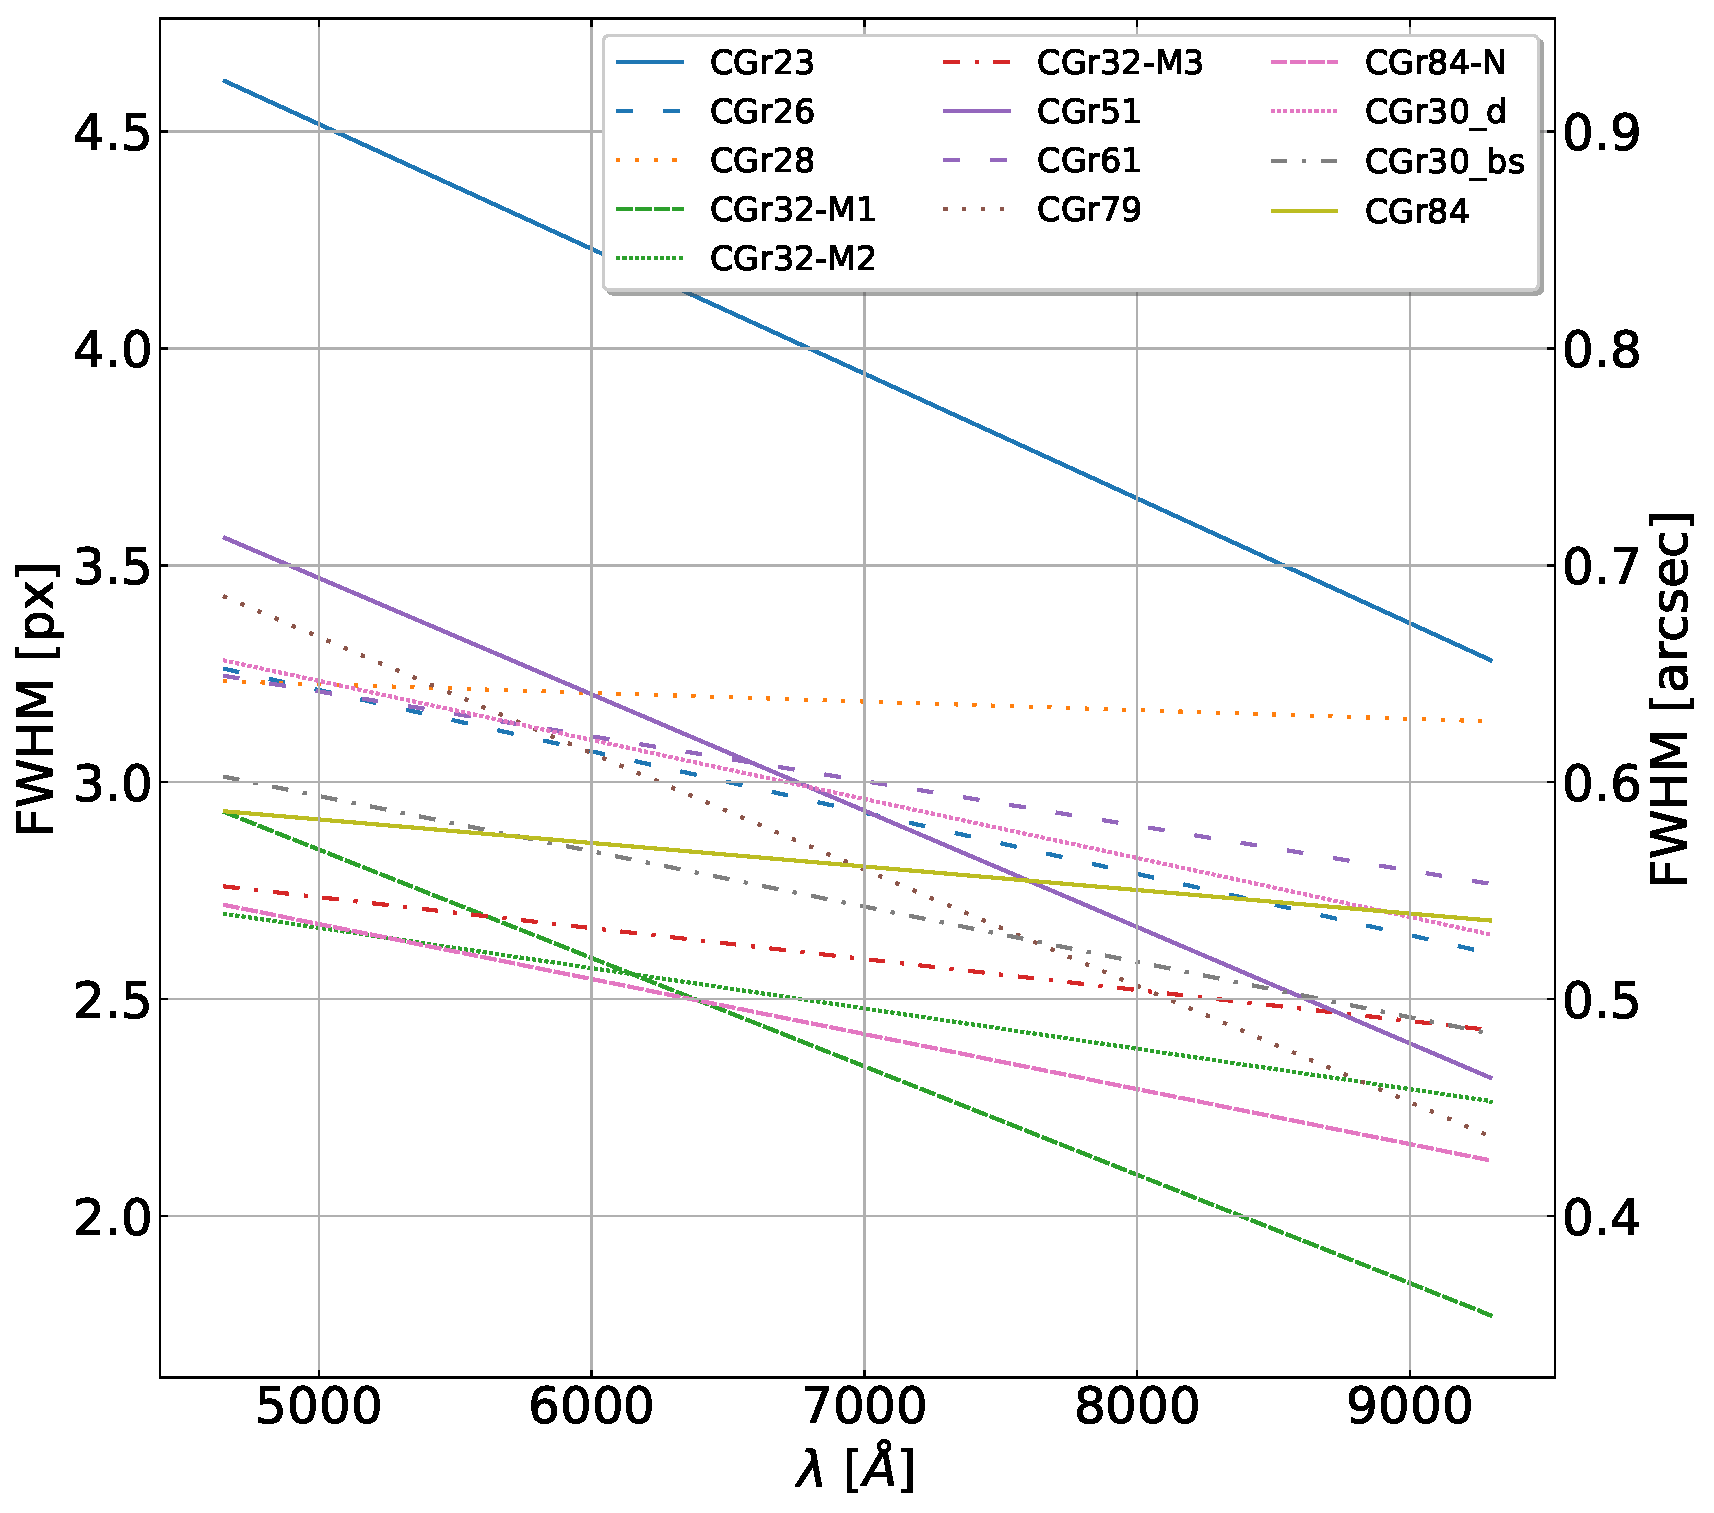
\includegraphics[width=\linewidth]{../Plots/FWHM_variation_with_lambda.pdf}
	\caption[PSF FWHM variation with wavelength.]{PSF $\rm{FWHM}$ variation with wavelength for the 16 MUSE fields (including \textit{best\_seing} and \textit{deep} observations) measured by V. Abril Melgajero and B. Epinat (LAM, Marseille). At least two values of the $\rm{FWHM}$ were derived from stars in the MUSE fields by fitting a Gaussian profile onto their light profile. We assumed a linear evolution with wavelength. Strong variations appear depending on the observed field.}
	\label{fig:FWHM_var_lambda}
\end{figure}